% Options for packages loaded elsewhere
\PassOptionsToPackage{unicode}{hyperref}
\PassOptionsToPackage{hyphens}{url}
%
\documentclass[
]{article}
\usepackage{amsmath,amssymb}
\usepackage{setspace}
\usepackage{iftex}
\ifPDFTeX
  \usepackage[T1]{fontenc}
  \usepackage[utf8]{inputenc}
  \usepackage{textcomp} % provide euro and other symbols
\else % if luatex or xetex
  \usepackage{unicode-math} % this also loads fontspec
  \defaultfontfeatures{Scale=MatchLowercase}
  \defaultfontfeatures[\rmfamily]{Ligatures=TeX,Scale=1}
\fi
\usepackage{lmodern}
\ifPDFTeX\else
  % xetex/luatex font selection
\fi
% Use upquote if available, for straight quotes in verbatim environments
\IfFileExists{upquote.sty}{\usepackage{upquote}}{}
\IfFileExists{microtype.sty}{% use microtype if available
  \usepackage[]{microtype}
  \UseMicrotypeSet[protrusion]{basicmath} % disable protrusion for tt fonts
}{}
\makeatletter
\@ifundefined{KOMAClassName}{% if non-KOMA class
  \IfFileExists{parskip.sty}{%
    \usepackage{parskip}
  }{% else
    \setlength{\parindent}{0pt}
    \setlength{\parskip}{6pt plus 2pt minus 1pt}}
}{% if KOMA class
  \KOMAoptions{parskip=half}}
\makeatother
\usepackage{xcolor}
\usepackage[margin=1in]{geometry}
\usepackage{graphicx}
\makeatletter
\def\maxwidth{\ifdim\Gin@nat@width>\linewidth\linewidth\else\Gin@nat@width\fi}
\def\maxheight{\ifdim\Gin@nat@height>\textheight\textheight\else\Gin@nat@height\fi}
\makeatother
% Scale images if necessary, so that they will not overflow the page
% margins by default, and it is still possible to overwrite the defaults
% using explicit options in \includegraphics[width, height, ...]{}
\setkeys{Gin}{width=\maxwidth,height=\maxheight,keepaspectratio}
% Set default figure placement to htbp
\makeatletter
\def\fps@figure{htbp}
\makeatother
\setlength{\emergencystretch}{3em} % prevent overfull lines
\providecommand{\tightlist}{%
  \setlength{\itemsep}{0pt}\setlength{\parskip}{0pt}}
\setcounter{secnumdepth}{-\maxdimen} % remove section numbering
% definitions for citeproc citations
\NewDocumentCommand\citeproctext{}{}
\NewDocumentCommand\citeproc{mm}{%
  \begingroup\def\citeproctext{#2}\cite{#1}\endgroup}
\makeatletter
 % allow citations to break across lines
 \let\@cite@ofmt\@firstofone
 % avoid brackets around text for \cite:
 \def\@biblabel#1{}
 \def\@cite#1#2{{#1\if@tempswa , #2\fi}}
\makeatother
\newlength{\cslhangindent}
\setlength{\cslhangindent}{1.5em}
\newlength{\csllabelwidth}
\setlength{\csllabelwidth}{3em}
\newenvironment{CSLReferences}[2] % #1 hanging-indent, #2 entry-spacing
 {\begin{list}{}{%
  \setlength{\itemindent}{0pt}
  \setlength{\leftmargin}{0pt}
  \setlength{\parsep}{0pt}
  % turn on hanging indent if param 1 is 1
  \ifodd #1
   \setlength{\leftmargin}{\cslhangindent}
   \setlength{\itemindent}{-1\cslhangindent}
  \fi
  % set entry spacing
  \setlength{\itemsep}{#2\baselineskip}}}
 {\end{list}}
\usepackage{calc}
\newcommand{\CSLBlock}[1]{\hfill\break\parbox[t]{\linewidth}{\strut\ignorespaces#1\strut}}
\newcommand{\CSLLeftMargin}[1]{\parbox[t]{\csllabelwidth}{\strut#1\strut}}
\newcommand{\CSLRightInline}[1]{\parbox[t]{\linewidth - \csllabelwidth}{\strut#1\strut}}
\newcommand{\CSLIndent}[1]{\hspace{\cslhangindent}#1}
\ifLuaTeX
  \usepackage{selnolig}  % disable illegal ligatures
\fi
\usepackage{bookmark}
\IfFileExists{xurl.sty}{\usepackage{xurl}}{} % add URL line breaks if available
\urlstyle{same}
\hypersetup{
  pdftitle={A guided tutorial on the generation of Raven-like matrices with the matRiks package},
  hidelinks,
  pdfcreator={LaTeX via pandoc}}

\title{A guided tutorial on the generation of Raven-like matrices with
the \texttt{matRiks} package}
\author{}
\date{\vspace{-2.5em}}

\begin{document}
\maketitle
\begin{abstract}
Few resources are available for the automatic generation of Raven-like
matrices. Some of them are no longer working, while others are hardly
customizable without adavnced programming skills. Although an R package
exists for generating stimuli for psychological assessments, it is
currently confined to create rotation of the same shape. The matRiks
package has been developed with the aim of overcoming the above
mentioned issues. This package generates matrices according to dufferent
types of rules, from the most basic ones based on the visuo spatial
features of the figures to the most complex ones, based on inferential
and inductive reasoning. This unveils the possibility of generating new
customizable stimuli and of systematically manipulating the complexity
of the stimuli. Being developed within the R environment, the matRiks
package is completely open-source, allows for the reproducibility of the
stimuli, and it can be easily used by people with basic knowledge of the
R language.
\end{abstract}

\setstretch{1.5}
\section{Introduction}\label{introduction}

Cattell (1963) defined fluid intelligence (\emph{g}) as the ability of
solving novel reasoning problems that has little to do with concepts
learned in schools or through acculturation processes. The adjective
``fluid'' explicitly refers to its ability to ``flow'' into a variety of
tasks and cognitive activities (Horn 1972). Given this definition of
fluid intelligence, it appears natural that the instruments used for its
evaluation tap on the respondent's ability to solve abstract problems
that involve acculturation as little as possible, such as figurative
analogies, figure classifications, matrices, and number and letter
series (Horn 1968).

The Raven's progressive matrices {[}RPM; JC ea Raven (1938){]} are among
the most famous tools for the assessment of \emph{g}. The RPM consists
in a series of non-verbal multiple-choice stimuli where respondents are
required to complete a series of drawings composed of different figures
by identifying the relevant features that rule the relationships between
the figures. These drawings are often referred to as matrices. To pursue
this aim, the respondents must choose the figure that complete the
drawing among a list of other figures, the so-called distractors. This
task should measure the ability of the respondents to identify and take
into account the features (also called ``rules'') that govern the
relationship between the figures to compose the drawing. Different
versions of the RPM exist, according to the target population (i.e.,
children with less then 12 years of age or adults) to which they are
administered. The Colored Progressive Matrices (CPM, J. Raven and Raven
1998) are composed of sets of \(2\times2\) matrices (i.e., 4-cell
matrices), some of which (CONTROLLARE) includes colored figures. The
advanced progressive matrices (APM, J. C. Raven 1962) are composed of
sets of \(3\times3\) matrices meant for assessment in gifted population
(DIRE MEGLIO). Finally, the RPM are meant for the assessment among the
general population and are composed of both \(2\times2\) and
\(3\times3\) matrices. The colored figures are present only in the CPM.

The RPM and similar tasks (here denoted as Raven-like matrices or
Raven-like tasks) are employed in different fields, from clinical
evaluation of intelligence to the selection processes in organizational
psychology (citation needed). Since Raven's and Raven-like tasks involve
the ability to solve new abstract problems, the stimuli composing these
tasks should not be spread among the general population to preserve the
novelty of the tasks. The rules that govern the relationship between the
figures of a matrix can also be used to generate new stimuli, and
different resources have been developed throughout the years with this
specific aim, such as Sandia (Matzen et al. 2010), Corvus (Thimbleby
2018), and the R package \texttt{IMak} (Blum and Holling 2018).

The stimuli generated with Sandia have been analysed in an Item Response
Theory framework to validate them as a test for measuring fluid
intelligence (Harris et al. 2020). The stimuli are available upon
request to the authors, however no new stimuli can be generated because
the code on which Sandia is based is no longer maintained. Corvus
represents another possible resource for generating Raven-like tasks.
Corvus is written in Javascript but the Author provided a nice and
easy-to-use graphical interface where the user can specify the figures
and the rule(s) for the generation of the matrices. However, Corvus
provides few degrees of freedom in terms of both the figures and the
number of rules that can be manipulated through the graphical interface.
Any customization from the user, like adding other figures, modifying
existing ones, or implementing new rules, require to modify the
JavaScript code, which might be quite demanding for people with little
to null experience in JavaScript coding. Finally, the \texttt{IMaK}
package is an \texttt{R} package that allows for generating visual
analogies. The code for generating such stimuli (along with their
response options) is quite straightforward and easy to use. However, the
stimuli that can be generated with the \texttt{IMaK} package are mostly
based on the rotation of the same figure to which some objects can be
added or removed. As such, the only rule that is manipulated is the
spatial rotation of the figures.

Given the limitations of the existing resources for generating
Raven-like tasks, there is the need of an open-source, easy-to-use, and
constantly maintained resource for generating such stimuli through the
systematic manipulation of rules applied to different figures. The
\texttt{matRiks} package (matRiks) has been developed to pursue these
aims. The package enables the generation of matrices by manipulating one
or multiple rules on one or multiple figures. Additionally, it
automatically generates the response list associated with the matrix.
Beyond the default settings, the matRiks package allows for the
generation of new figures and customization of matrices and response
lists. The systematic manipulation of both the rules and the figures for
the matrix generation should grant the possibility of grading the
granularity of the complexity of the matrices by varying one element at
the time. In a similar vein, the package should allow for generating
matrices that can be considered equivalent in terms of rules employed
for their generation but that differ in terms of figures composing the
drawing. In what follows, the term stimulus is used to identify the
matrix with its associated response list.

The manuscript is organized as follows. The next section presents the
rules that are usually employed in the RPM along with the specific types
of error responses (i.e., distractors) that compose the response list
associated with a matrix. A complete example of the generation of a
stimulus (i.e., the matrix and the associated response list) and some
final remarks on the potential applications of this package conclude the
presentation.

\section{Background}\label{background}

\subsubsection{Rule based matrices}\label{rule-based-matrices}

Literature highlights a plethora of rules that can be manipulated for
the generation of the Raven-like tasks (cit cit cit). Some of the rules
have different names, but they do refer to the same manipulation. For
instance, the rule defined as ``and problem'' in Harris el a. 2020 is
called ``intersection'' rule in Arendasy et al.~2005. CONTROLLA IL PAPER
SE LA REGOLA E' CORRETTA E LE CITAZIONI SONO CORRETTE.

they can be summarized into different macro-categories, namely
visuospatial rules (i.e., the manipulation concerns the graphical and
spatial features of the figures, Figure @ref(fig:visuoRule)), and
logical rules (i.e., the manipulation concerns the logical relationships
between the figures composing the matrix, Figure @ref(fig:logiRule)).
The rules can be used to manipulate different figures to generate a
matrix.

\begin{figure}

{\centering 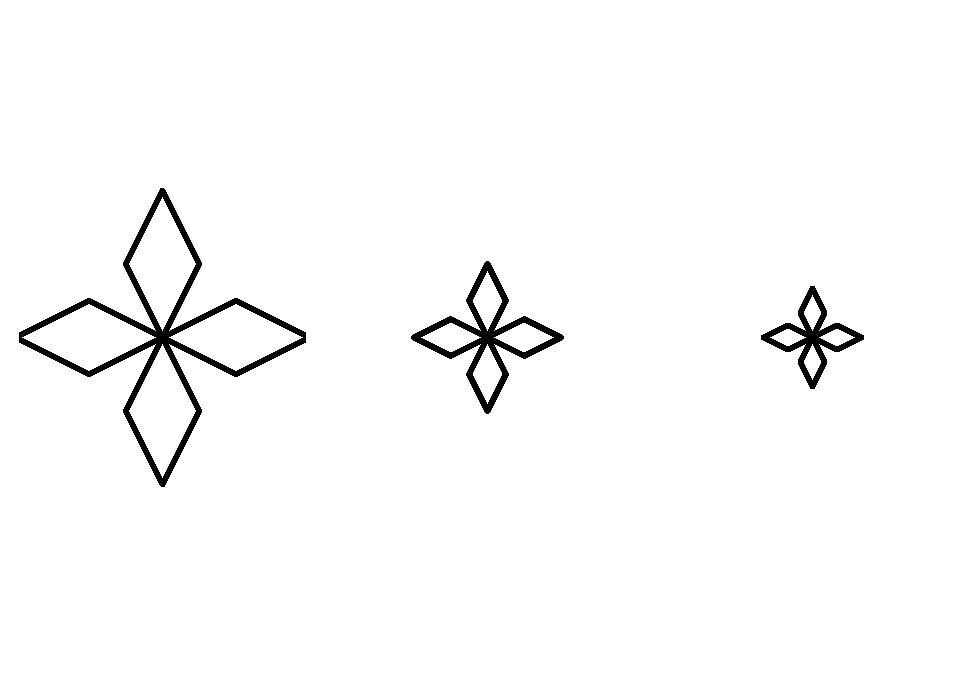
\includegraphics[width=0.7\linewidth]{paper-pdf_files/figure-latex/visuoRule-1} 

}

\caption{Example of visuospatial rule: Changes in size}\label{fig:visuoRule}
\end{figure}

\begin{figure}

{\centering 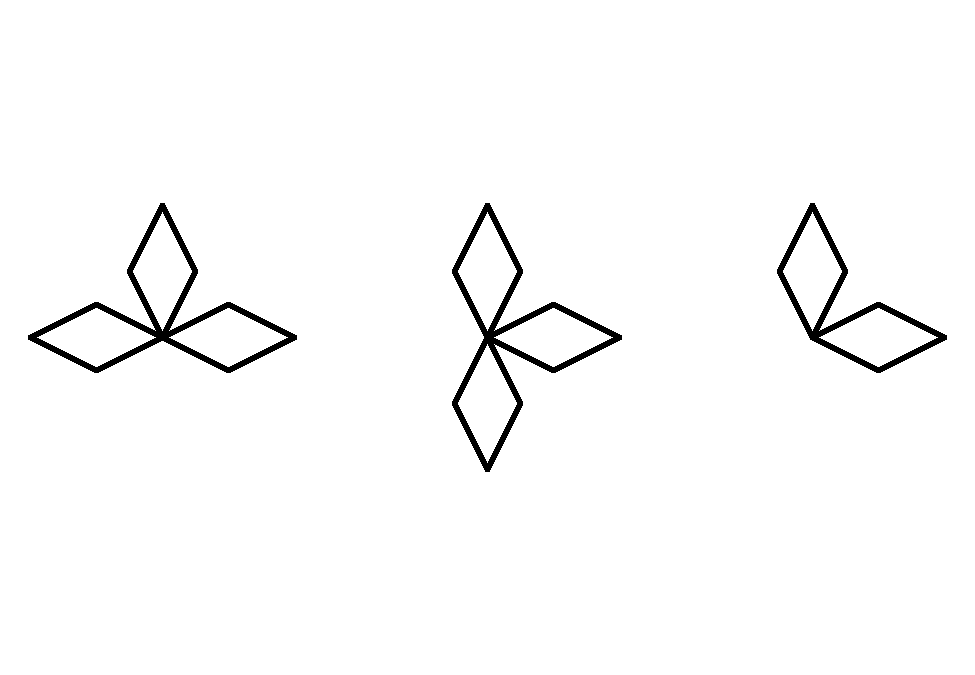
\includegraphics[width=0.7\linewidth]{paper-pdf_files/figure-latex/logiRule-1} 

}

\caption{Example of logical rule: Insiemistic Interscetion AND}\label{fig:logiRule}
\end{figure}

In Figure @ref(fig:visuoRule), the manipulation concerns a specif
feature of the figure, that is its size, and it can be observed as the
the figure decreases its size across the cells. The leftmost cell
contains the figure with its original size, the middle cell contains a
smaller figure, while the rightmost cells contains the smallest one. In
Figure @ref(fig:logiRule), the manipulation concerns the relationships
between the objects composing the figures, which are combined together
according to a logical rule based on the insiemistic intersection of the
objects. Specifically, the figure in the rightmost cell results from the
intersection between the figures in the leftmost cell and those in the
middle cell.

Both visuospatial and logical rules can be manipulated according to
directional logic. Specifically, the rules can be applied horizontally
(i.e., the manipulation of the rule can be seen across columns but not
across rows, H direction), vertically (i.e., the manipulation of the
rule can be seen across rows but not across columns, V direction), or
diagonally (i.e., the manipulation of the rule can be seen both across
columns and across rows). Concerning the diagonal directional logic, it
can follow either the main diagonal of the matrix (i.e., the
manipulation of the rule can be seen from the top-left corner to the
low-right corner, TL-LR direction) or the secondary diagonal of the
matrix (i.e., the manipulation of the rule can be seen from the low-left
corner to the top-right corner, LL-TR direction).

\subsubsection{The response options}\label{the-response-options}

A large corpus of literature has investigated the role of the
distractors in the response processes involved when solving the Raven
matrices, focusing on the specific error responses chosen by the
respondent (fort, kunda, storme). The underlying logic is that the
incorrect response is not chosen at random by the respondent, but it can
be the result of an educated guess, or it can be chosen because the
respondent is misled by a specific feature. In other words, the
incorrect responses might reflect an incorrect solution strategy
resulting in the choice of a specific type of distractor over another
one (Kunda et al. 2016). The distractors can be classified according to
the incorrect response strategy they represent. Kunda et al. (2016)
present a list of criteria for the identification of the distractors in
the SPM based on classification of the error types from the CPM and APM
manuals (John Raven and Raven 2004). The distractor that is chosen in
place of the correct response option can be collected into four main
four conceptual errors: (i) Repetition (R) errors occur when the chosen
response option is a cell adjacent to the blank space, (ii) Difference
(D) errors occur when the chosen response option is completely different
from any entry of the matrix, (iii) Wrong Principle (WP) errors occur
when the chosen response option follows rules other than the ones used
in the matrix, and (iv) Incomplete Correlate (IC) errors occur when the
chosen response option is in fact the correct response with a variation
on a single feature.

The characteristics of the specific error response can be categorized in
various ways. For example, the repetition category can be divided based
on the position of the repeated cell relative to the blank cell. Three
error types within the R category can be identified: R-Left, R-Top, and
R-Diagonal, depending on whether the repeated cell is to the left,
above, or diagonally aligned with the blank cell.

Regarding the wrong principle macro category, some specific error types
might involve the repetition of a cell that is not adjacent to the blank
space (e.g., WP-Copy) or the combination of elements from different
cells in a way that does not follow the rules used for creating the
matrix.

Some specific errors in the incomplete correlate macro category include
changes to the orientation of the correct response (i.e., IC-flip),
changes in the color of the correct response (i.e., IC-Neg), changes in
the size of the correct response (i.e., IC-Size), or the omission of an
element from the correct response (i.e., IC-Inc).

Finally, regarding the difference macro category, specific errors might
include a cell being completely white or black (D-Blank) or the merging
of different cells within the matrix (D-Union).

The criteria for the classification of the error types were used for the
formal definition and generation of the distractors implemented in the
\texttt{matRiks} package. These criteria were included in the response
options operator with the aim of providing the user with a response list
composed of 11 elements (ten distractors and the correct response) among
which they could choose the most appropriate ones. Specifically, the
response options operator generates a response list composed of the
correct response, three reptition distractors, one difference
distractor, two wrong principle distractors, and four incomplete
correlate distractors. Further details on the formal definition of each
of the distractors and on their generation are given in the ``Generation
of the response list'' Section.

\section{The matRiks package}\label{the-matriks-package}

The \texttt{matRiks} package (Brancaccio, Epifania, and de Chiusole
2023) can generate \(2 \times 2\) and \(3 \times 3\) Raven-like matrices
with their corresponding set of responses (i.e., the correct response
and all the distractors described in the Generation of response list
section). The Raven-like matrices are generated according to either
visuospatial or logic rules, which can be concatenated with three
different directional logic, namely vertically, horizontally, and
diagonally. Finally, it is possible to print the generated matrices and
set of distractors as either single images (i.e., each cell of the
matrix and each distractor are printed separately) or as a complete
figure with the set of single distractors.

\phantomsection\label{refs}
\begin{CSLReferences}{1}{0}
\bibitem[\citeproctext]{ref-Blum2018}
Blum, Diego, and Heinz Holling. 2018. {``Automatic Generation of Figural
Analogies with the IMak Package.''} \emph{Frontiers in Psychology} 9
(1286): 1--13. \url{https://doi.org/10.3389/fpsyg.2018.01286}.

\bibitem[\citeproctext]{ref-matRiks}
Brancaccio, Andrea, Ottavia M. Epifania, and Debora de Chiusole. 2023.
\emph{matRiks: Generates Raven-Like Matrices According to Rules}.
\url{https://CRAN.R-project.org/package=matRiks}.

\bibitem[\citeproctext]{ref-cattell1963}
Cattell, Raymond B. 1963. {``Theory of Fluid and Crystallized
Intelligence: A Critical Experiment.''} \emph{Journal of Educational
Psychology} 54 (1): 1.
https://doi.org/\url{https://doi.org/10.1037/h0046743}.

\bibitem[\citeproctext]{ref-harris2020}
Harris, Alexandra M, Jeremiah T McMillan, Benjamin Listyg, Laura E
Matzen, and Nathan Carter. 2020. {``Measuring Intelligence with the
Sandia Matrices: Psychometric Review and Recommendations for Free
Raven-Like Item Sets.''} \emph{Personnel Assessment and Decisions} 6
(3): 6.

\bibitem[\citeproctext]{ref-horn1968}
Horn, John L. 1968. {``Organization of Abilities and the Development of
Intelligence.''} \emph{Psychological Review} 75 (3): 242.

\bibitem[\citeproctext]{ref-horn1972}
---------. 1972. {``The Structure of Intellect: Primary Abilities.''}
\emph{Multivariate Personality Research}, 451--511.

\bibitem[\citeproctext]{ref-kunda}
Kunda, Maithilee, Isabelle Soulières, Agata Rozga, and Ashok K. Goel.
2016. {``Error Patterns on the {Raven}'s {Standard} {Progressive}
{Matrices} {Test}.''} \emph{Intelligence} 59 (November): 181--98.
\url{https://doi.org/10.1016/j.intell.2016.09.004}.

\bibitem[\citeproctext]{ref-matzen2010}
Matzen, Laura E, Zachary O Benz, Kevin R Dixon, Jamie Posey, James K
Kroger, and Ann E Speed. 2010. {``Recreating Raven's: Software for
Systematically Generating Large Numbers of Raven-Like Matrix Problems
with Normed Properties.''} \emph{Behavior Research Methods} 42 (2):
525--41.

\bibitem[\citeproctext]{ref-raven1938}
Raven, JC ea. 1938. {``Raven's Progressive Matrices.''} \emph{Western
Psychological Services} 2: 5.

\bibitem[\citeproctext]{ref-raven1962}
Raven, John C. 1962. {``Advanced Progressive Matrices: Sets i and II.''}
London:H.K. Lewis.

\bibitem[\citeproctext]{ref-raven2004}
Raven, John, and H. Raven. 2004. {``Manual for {Raven}'s {Progressive}
{Matrices} and {Vocabulary} {Scales}, {Section} 3: {The} {Standard}
{Progressive} {Matrices}, {Including} the {Parallel} and {Plus}
{Versions}. 2000 {Edition}, Updated 2004.''} In, Section 3.

\bibitem[\citeproctext]{ref-raven1998}
Raven, J, and JC Raven. 1998. {``Court h. Coloured Progressive Matrices.
1998 Edition.''} USA: Harcourt Assesment.

\bibitem[\citeproctext]{ref-thimbleby2018}
Thimbleby, Isaac James. 2018. {``Corvus: An Automatic Raven's-Like Test
Generator.''} PhD thesis, University of Oxford.

\end{CSLReferences}

\end{document}
